\chapter{Machine learning on referring epxressions}
\label{chap:ml}
REs are big part of language generation of a navigation system and especially so in the GIVE scenario. My work attempts to apply machine learning techniques to the S-GIVE dataset with the goal to help the navigation system with REG. These attempts are presented in this chapter.

Machine learning (ML) is becoming a popular topic together with a very broad term of Big Data. This branch of artificial intelligence encompasses various problems such as classification or clustering. Research in the area of ML spawned various algorithms for solving these problems and evaluation techniques for comparing the models outputted by the learning process. 

It is important to emphasize that ML creates models which can only be as good as the data they were trained on. Careful and thorough data analysis is crucial part of the ML process. When it comes to feature extraction, experimentation are sometimes the only methods for finding better models. 

The first section serves as an analysis of the S-GIVE dataset.

In the second section I will describe attempts at predicting the timing of the first reference to a target button. 

The third section talks about modeling chains of references. 

The fourth section briefly touches on the topic of using room memory. 

In the last section, I will present my thoughts on the results of the previous sections.

\section{S-GIVE dataset analysis}

\subsection{World and Demographic factors}
\label{subsec:world-demo-factors}
As was noted repeatedly in Chapter \ref{chap:give-challenge}, the world had significant influence on the task success rate in GIVE Challenge. However in the GIVE Challenge the worlds were designed to be of a different difficulty, whereas in the S-GIVE dataset they were designed to be similar in terms of the difficulty to minimize effects outside of the navigation strategy. In addition, all the sessions were successful except for one which was discarded. The question about the influence of the worlds must be reformulated, since the task success rate no longer makes sense. Instead, I will measure task performance by time required to finish the task (duration) and also use other performance measure when appropriate.

Despite the design choices, I found that the normal worlds 1 and 3, had a significantly different mean duration (p-value $0.0473$ for unpaired two-sample t-test). There are multiple explanation for this difference. The relatively small number of subjects is certainly one of them. We can also notice in Figure \ref{fig:dataset-world3} slightly complicated system of hallways in the center of world-3. But this discovery does not have a major influence on my work. Moreover, the difficult worlds did not have significant difference between their mean duration (p-value $0.6195$ for unpaired two-sample t-test).

Another thing I was interested in was the influence of the gaming experience of both participants on certain performance measures, namely on the duration, on the average speed of IF movement and the time the IF spent moving. The average speed of the IF is simply a total distance the avatar controller by IF travelled in a session divided by the duration. The time the IF spent moving aggregates the time where avatar wasn't either motionless or wasn't only rotating in place. 

I found correlations between gaming experience and these variables. Table \ref{tab:demfactors-gaming} shows the correlation matrix between gaming experience and performance measure.  Not surprisingly, these correlation are especially high for the IF, since he/she is the one who is actually playing the world, but the IG gaming experience seems to have some effect as well. The past gaming experience (questions 7 in third part of the questionnaire) is more important than contemporary playing (question 6 in the third part of the questionnaire). Most prominent are the familiarity of IF with 3D games (question 5),  the IF hours per week spent playing games at the past peak gaming period (question 7), the same variable for IG and hours spent gaming per week for IF at present (question 6). For the difficult worlds some correlations change slightly. IF's gaming at past peak period has much weaker correlation with duration here. In general, individuals who are familiar with games (gamers) take less time to finish the world, they spent more time moving and they have higher speed.


\begin{table}[!htbp]
 \centering
\begin{tabular}{llccc}
\toprule
World & Question  & Duration & Speed & Time moving  \\
\midrule
Normal 	& IF hours/week peak gaming (7) 	& -0.411 &	0.486 &	0.428\\
 		& IF hours/week now 	(6)			& -0.366	 & 	0.338 &	0.255\\
 		& IF familiarity 3D games (5)	& -0.590	 &	0.720 &	0.664\\
 		& IG hours/week peak gaming (7) 	& -0.359 &	0.450 &	0.435\\
 		& IG hours/week now 	(6)			& 0.079	 &	0.155 &	0.180\\
 		& IG familiarity 3D games (5)	& -0.230 &	0.221 &	0.224\\
\midrule
Difficult& IF hours/week peak gaming (7) & 0.111 &	0.199 &	0.135\\
 		& IF hours/week now (6)			& -0.388 &	0.312 &	0.233\\
 		& IF familiarity 3D games (5)	& -0.478 &	0.569 &	0.520\\
 		& IG hours/week peak gaming (7) 	& -0.287 &	0.715 &	0.715\\
 		& IG hours/week now (6)			& 0.149 &	0.348 &	0.420\\
 		& IG familiarity 3D games (5)	& 0.009 &	0.403 &	0.473\\
\bottomrule
\end{tabular}
\caption{Correlation matrix of gaming experiences and performance measures}
\label{tab:demfactors-gaming}
\end{table}

I also looked at the influence of SBSOD scores (second part of the questionnaire) on the task proficiency. A correlation matrix revealed weak or almost no correlation between SBSOD scores and the time needed to complete the world, as can be seen in Table \ref{tab:demfactors-sbsod}. In the difficult worlds, however, the correlation became slightly stronger.

\begin{table}[!htbp]
 \centering
\begin{tabular}{llc}
\toprule
 World & Role   & Duration \\
\midrule
Normal & IF &	-0.085\\
 & IG &	-0.082\\
\midrule
Difficult & IF & 0.162\\
 & IG &	-0.210\\
\bottomrule
\end{tabular}
\caption{Correlation between SBSOD scores and duration}
\label{tab:demfactors-sbsod}
\end{table}

The data suggest that there is positive correlation between male gender and task proficiency measured as duration. Table \ref{tab:demfactors-gender} shows these correlations. There are several facts to take in consideration here. This correlation might have been caused by having more male gamers than female gamers. In fact, Table \ref{tab:demfactors-gender-fam} suggest so. There has also been research about influence of gender on spatial cognition and mental rotation; an example of more recent one is \citep{geary2000sex}. They conclude that males are more proficient in tasks requiring mental rotation. Since the IGs have to do mental rotation while giving direction in GIVE scenario, this might be a source of the correlation. Another paper worth considering on this topic is \citep{moffat1998navigation}, which found a gender difference in time required to finish a virtual maze. However, when statistically compared the differences are not significant. For the IF the p-value of Welch two sample t-test is 0.083. For the IG the p-value of Welch two sample t-test is 0.230.

\begin{table}[!htbp]
 \centering
\begin{tabular}{llc}
\toprule
 World & Role   & Duration \\
\midrule
Normal & IF &	-0.234\\
 & IG &	-0.277\\
\midrule
Difficult & IF & -0.349\\
 & IG &	-0.106\\
\bottomrule
\end{tabular}
\caption{Correlation between male gender and duration}
\label{tab:demfactors-gender}
\end{table}

\begin{table}[!htbp]
 \centering
\begin{tabular}{lc}
\toprule
Role    & Familiarity with 3D games \\
\midrule
 IF &	 0.341\\
 IG &	0.661\\
\bottomrule
\end{tabular}
\caption{Correlation between male gender and familiarity with 3D games}
\label{tab:demfactors-gender-fam}
\end{table}

Table \ref{tab:demfactors-age} shows correlation matrix for age. The age of the IF has a positive correlation with task proficiency measured in duration, and in difficult worlds this correlation is one of the strongest ones. Older IF are also moving less and are generally slower. For IG the correlations have the same direction, however they are much weaker. However the relationship between age and gaming experience is worth considering in this case, so Table \ref{tab:demfactors-gaming-age} shows correlations between them. We can see that the correlation is present but not that strong.

\begin{table}[!htbp]
 \centering
\begin{tabular}{llccc}
\toprule
World & Role  & Duration & Speed & Time moving  \\
\midrule
Normal 	& IF & 0.175 & -0.467 & -0.448\\
 		& IG & 0.275 & -0.098 & -0.125\\
\midrule
Difficult& IF & 0.614 &	-0.275 &-0.196\\
 		& IG  & 0.016 &	-0.217 &-0.232\\
\bottomrule
\end{tabular}
\caption{Correlation matrix of age and performance measures}
\label{tab:demfactors-age}
\end{table}


\begin{table}[!htbp]
 \centering
\begin{tabular}{lc}
\toprule
 Question  & Age\\
\midrule
Hours/week peak gaming (7) 	& -0.199 \\
Hours/week now 	(6)			& -0.269	\\
Familiarity 3D games (5)	& -0.380	 \\ 
\bottomrule
\end{tabular}
\caption{Correlation matrix of gaming experiences and age}
\label{tab:demfactors-gaming-age}
\end{table}

Lastly I was interested how familiarity of participants with each other (questions 9-12 in the third part) influenced the task performance. Table \ref{tab:demfactors-famother} shows, that, unexpectedly, knowing the partner had a negative impact on task efficiency. The most correlated question was question 10: how well they know each other.

\begin{table}[!htbp]
 \centering
\begin{tabular}{llc}
\toprule
World & Question  & Duration \\
\midrule
Normal 	& IF Co-players in past (12) 	& -0.038\\
 		& IF Collaborative work 	(11)		& 0.109	 \\
 		& IF how well know each other (10)		& 0.529\\
 		& IF know each other (9)			& 0.164	\\
 		& IG Co-players in past (12) 	& -0.124\\
 		& IG Collaborative work 	(11)		& 0.189	 \\
 		& IG how well know each other (10)		& 0.420\\
 		& IG know each other (9)			& 0.177	\\ 		
\midrule
Difficult& IF Co-players in past (12) 	& -0.078\\
 		& IF Collaborative work 	(11)		& 0.170	 \\
  		& IF how well know each other (10)		& 0.437\\
 		& IF know each other (9)			& 0.247	\\
 		& IG Co-players in past (12) 	& 0.291\\
 		& IG Collaborative work 	(11)		& 0.245	 \\
 		& IG how well know each other (10)		& 0.361\\
 		& IG know each other (9)			& 0.189	\\
\bottomrule
\end{tabular}
\caption{Correlation between participants familiarity and duration}
\label{tab:demfactors-famother}
\end{table}

After exploring interesting correlations, I will now focus on RE.

\subsection{Referring expressions analysis}
Because REs are the main focus of my research, this subsection serves as a brief introductory analysis of REs in the S-GIVE dataset.

Overall, 793 REs were annotated in the manual annotations. Apart from the time interval of the reference, several other facts were annotated in the manual annotations, as was mentioned in Chapter \ref{chap:s-give}. First of all, the target button of each RE was annotated. The count of distinct target buttons is 29.  

REs were also separated into 5 high-level categories depending on what is the target of the reference. The  overview of the categories is in the following list:

\begin{itemize}
\item
Target - Referring to the target button
\item
Group - Referring to a group of buttons, one of which is the target button
\item
Landmark object - Referring to a landmark (any object or room feature, but not a button) which will then be used to locate the target button
\item
Landmark button - Referring to a distractor button as a landmark
\item
Remove button -  Referring to a distractor button to exclude it
\end{itemize}

The percentage count of the categories is given in Table \ref{tab:res-groups}. References to target buttons are a dominant category. Around 10\,\% of the references are group references. References to landmarks occupy only 6\,\% of all references.

\begin{table}[!htbp]
 \centering
\begin{tabular}{lr}
\toprule
Category  & Percentage (\%)  \\
\midrule
Target   		& 82.47\\
Group 			& 10.34\\
Landmark object 	& 5.04\\
Landmark button	& 1.39\\
Remove button 	& 0.76\\
\bottomrule
\end{tabular}
\caption{Percentage of REs in the categories}
\label{tab:res-groups}
\end{table} 

Another layer of manual annotations looked into the content of the REs. It was done through annotating several semantic elements of the REs of the Target category. They are listed in the following list and their usage is summarised in Table \ref{tab:res-contents}. Please note that these elements are not necessarily exclusive with each other.

\begin{itemize}
\item
Type - RE expressed the target object as its type (``button'')
\item
One - RE expressed the target object as ``one''
\item
Pronoun - RE expressed the target object as a pronoun
\item
Color -  RE contained color of the target object
\item
Button location - RE contained relative location of the target object to a distracting button
\item
Object location - RE contained relative location of the target object to a distracting object (not a button)
\item 
IF location - RE contained relative location of the target object to the IF
\item
Room location - RE contained relative location of the target object to a room
\item
History - RE informed that the target object was already manipulated with
\end{itemize}

\begin{table}[!htbp]
 \centering
\begin{tabular}{lr}
\toprule
Element  & Percentage (\%)  \\
\midrule
Type   			& 55.35\\
Color			& 47.09\\
One 				& 26.29\\
Button location & 18.80\\
Object location 	& 16.67\\
IF location		& 11.62\\
Pronoun			& 10.70\\
History			& 6.88\\
Room location 	& 5.81\\
\bottomrule
\end{tabular}
\caption{Percentage of REs which contained a semantic element}
\label{tab:res-contents}
\end{table} 

From previous tables, we can see prevalence of relatively simple RE. However, the next subsection will show that the situation is more complex than it may seem from this subsection.

\subsection{Chains of references analysis}
\label{subsec:dataset-chains}
An interesting phenomenon I have noticed and further explored in the dataset are consecutive references to one button. It can be seen in the following sentences: ``Straight ahead of you there on the opposite wall there are two blue buttons. Press the one on the right. The one close to the picture.'' The IG started of with a references to a group of two buttons; the target button being one of those two. In the second sentence he picked out the target button from the group. In the last sentence the IG made another reference containing a landmark, adding redundant information. Since the references are concerned with one target button and follow each other relatively fast, I have called them chains of references (chains, in short). These chains are examples of non-standard referring strategy, I was mentioning since the beginning of this paper.

The chains vary in length, from short ones, consisting of only two references, up to lengthy ones with eight references following each other. The example from previous paragraph is three references long. Figure \ref{fig:chains_len_histo} shows a histogram of the chains' length.

\begin{figure}[!htbp]
  \centering
	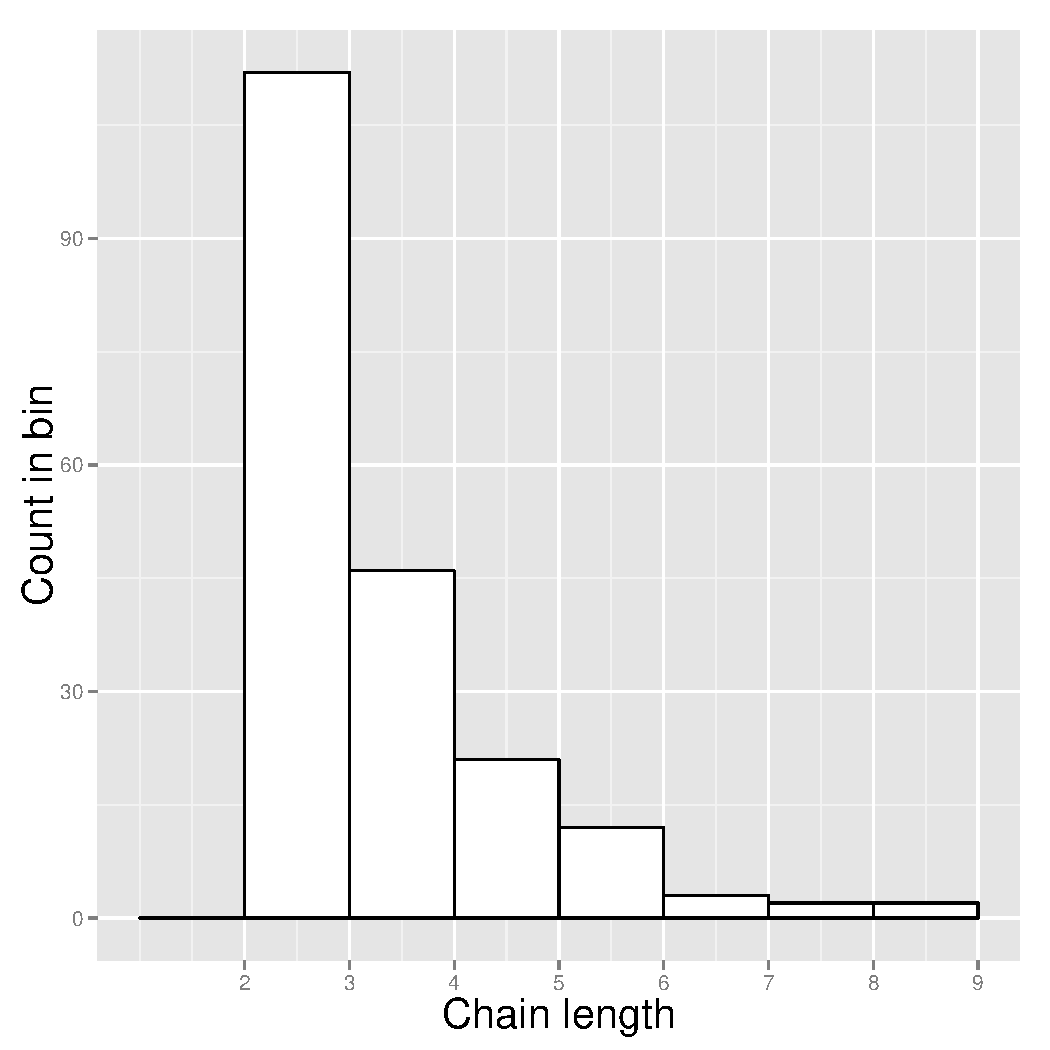
\includegraphics[width=0.6\textwidth]{Images/chains_len_histo}
	\caption{Histogram of the chain length}
	\label{fig:chains_len_histo}
\end{figure}

The chains are significant part of the discourse, in fact over 77\,\% of all RE belong to a chain. There is in total 198 chains in the dataset. However, the chains have multiple linguistic functions, which makes them difficult to explore. Even inside one chain, there are often combination of functions. I have manually annotated some common functions of the chains. The most common one is to inform the IF that he is supposed to press the target button. A simple example of this function, which I call action function, is in following discourse: ``The red button in front of you. Press that one.'' It may sound redundant to use action function as the experiment progresses, since the IF are not manipulating the buttons in any other way than pressing them. But I have found out that it's often the case, that IG still uses action functions in later stages of navigation.

Another common function is confirmation: ``That same red button we pressed before, we'll press that again. Yeah that one.'' The IG confirms at the end of the previous utterance that IF is looking at or heading to a correct target button.

The IG often utters a RE, which does not perfectly ``pick out'' the target button from the set of buttons in the room. The IG can make up for that information deficit with a confirmation or by further specifying with another RE. That is a specification function, as in following two sentences: ``Now that green button. You want the one closer to the lamp.''

When a group of buttons is utilized in a RE and the target button is part of that group, it is inevitable that the IG will have to make another RE to ``pick out'' the target button from the group. Therefore group references imply chains of references and should be considered as one of the functions. A simple example of the group function: ``Two blue buttons on the wall. Hit the blue button on the right side.''

When the IF has clearly chosen the wrong button, the IG will try to correct that error. I call that an error function. The following extract features this function: ``That blue button. No no no. The other. That one.''

A summary of the functions of all 198 chains, which I have manually annotated, is in Table \ref{tab:chains-functions}. Please note that these functions are not exclusive. One chain can have both a confirmation and a specification function.

\begin{table}[!htbp]
 \centering
\begin{tabular}{lr}
\toprule
Function   & Chains containing it (\%)  \\
\midrule
Action    		& 66.2\\
Confirmation	 	& 29.3\\
Specification 	& 25.3\\
Group 	  		& 24.7\\
Error 			& 11.1\\
\bottomrule
\end{tabular}
\caption{Percentage of chains having specific functions}
\label{tab:chains-functions}
\end{table}

These chains will be further explored in the following sections, but as one can already notice, they are complex language phenomenon.

\section{Timing of the first reference}
\label{sec:timing-firsref-ml}
The work of \citet{stoia2006sentence} was previously mentioned in the related work section of Chapter \ref{chap:bg}. They applied machine learning to the timing of the first reference in a 3D virtual world. The set-up of their experiment is quite similar to the GIVE scenario and so I decided it would be interesting to replicate their methodology on the GIVE dataset. 

I defined the problem of the timing of the first reference as a classification task, as did \citet{stoia2006sentence}. More precisely binary classification, the two classes being either refer to the target button or delay the reference. After extracting the first references to buttons which needed to be pressed from the dataset, I excluded plural references, because of their complexity. Some buttons were placed on top of each other and the IG wasn't sure which one need to be pressed. These were excluded as well because of the unnecessary confusion. In addition, some buttons were referred to multiple times, because they needed to be pressed twice. The later references may have a completely different structure and the buttons were therefore excluded. That left me with 351 first references. For each first reference I have chosen one negative example, where the IG could refer to the target but chose not to. I picked negative examples randomly from the interval between entering the room and the time of the first reference. The classification was therefore done in two time points for each target button, in a randomly selected point between entering the room and uttering the first reference and in moment of the uttering the first reference. Overall, it gives is 702 data-points with perfectly balanced classes.

As for features extraction, I have chosen similarly to \citet{stoia2006sentence} various spatial information. For the positive examples, I averaged these spatial information over a 0.6 seconds window centered on the time of the reference. The reasoning for that, is that the IG takes the scene situation into consideration before and possibly after they start uttering the reference. For negative examples I chose not to average them, since they are chosen randomly. All features are listed in the following list. The list also includes figure numbers. These figures are histograms of the attributes, separated for both classes and can be found in appendix.

\begin{itemize}
\item
Distance to target button - Figure \ref{fig:fref-distrib-dist}
\item
Absolute value of angle to target - Figure \ref{fig:fref-distrib-angle}
\item
Whether target is visible (True/False) - Figure \ref{fig:fref-distrib-visib}
\item
Number of distractors - Figure \ref{fig:fref-distrib-distractors}
\item
Number of distracting buttons - Figure \ref{fig:fref-distrib-distbuttons}
\item
Number of visible buttons with smaller angle to IF than the target button - Figure \ref{fig:fref-distrib-distangles}
\end{itemize}

Once I have extracted these features I used three machine learning techniques: C4.5 decision trees because of their easy interpretation, Naive Bayes to observe the effect of all attributes and Support vector machine for linear classification. I used the Weka software implementation of previous algorithms \citep{hall2009weka}.

For all the algorithms I used a standard ten-fold cross validation. The results can be seen in table \ref{tab:firstref}. A pruned decision tree for timing of the first reference can be seen in Figure \ref{fig:dectree}. I used two simple baselines to compare the results with. I have perfectly balanced classes so the first baseline is 50\,\%. A simple rule for the first reference is to refer when the target is visible, and delay it if the target is not visible. In my case that rule has an accuracy of 64.2\,\%. 

\begin{table}[!htbp]
 \centering
\begin{tabular}{lr}
\toprule
Model    & Accuracy (\%)  \\
\midrule
Class baseline    & 50.0\\
Visibility baseline & 64.2\\
\midrule
Naive Bayes  & \textbf{64.7} \\
C4.5 & 63.3 \\
SVM & 55.4 \\
\bottomrule
\end{tabular}
\caption{Results of first reference timing modeling}
\label{tab:firstref}
\end{table}

Only one algorithm was able to get over the visibility baseline and not by a significant amount. These results were surprising, because \citet{stoia2006sentence} had success with the same approach on a similar dataset. Reasons for this difference are probably in the differences between their experiment and the GIVE set-up. First, their tasks also included different actions than pushing buttons (e.g. picking up items). Second, their worlds had higher diversity of the distractors and smaller frequency of them. With increasing number of distractors and particularly distractors of the same category, it seems that spatial features loose their power in predicting the timing of the first reference. The number of visible distractors was the best attribute in their decision tree, but in my tree (Figure \ref{fig:dectree}) it had lower information gain. Moreover, the decision tree did the split on the number of visible buttons not the number of all visible distractors.

After the timing of the first references classification proved to be more difficult than expected, I have switched from predicting the timing of the references to predicting their content. I focused on the content of chains of references.

\begin{figure}[!htbp]
 \centering
\small
\begin{verbatim}
Distance to target <= 4.45
| Is target visible? = False: DELAY
| Is target visible? = True
| | Distance to target <= 2.51: REFER
| | Distance to target > 2.51
| | | Number of distracting buttons <= 4.67: REFER
| | | Number of distracting buttons > 4.67: DELAY
Distance to target > 4.45: DELAY
\end{verbatim}
\caption{Decision tree for first reference timing}
\label{fig:dectree}
\end{figure}

\section{Chains of references}
Subsection \ref{subsec:dataset-chains} introduced the phenomenon of chains of references. It also analysed various linguistic functions the chains can play in REG. This section will build on top of this analysis, by employing machine learning techniques to model the chains.

A valid and important question is whether chains aren't something, which should actually be avoided, instead of modelled. That is, what is the relation between usage of chains and task performance measure, such as the duration. To address this issues, I used linear regression predicting the duration of the experiment explained by the average chain length. I measured the goodness of fit of the model with the coefficient of determination ($R^2$), defined as:
\begin{equation*} 
R^2 = 1 - \frac{\sum_i (y_i - f_i)^2}{\sum_i (y_i - \hat{y})^2}\text{,}
\end{equation*}
where $y_i$ are observed values, $f_i$ are predicted values and $\hat{y}$ is a mean of the observed values.

Figure \ref{fig:chains_dur_scatter} does contain a hint of a trend, but also contains a lot of counter-examples. 

\begin{figure}[!htbp]
  \centering
	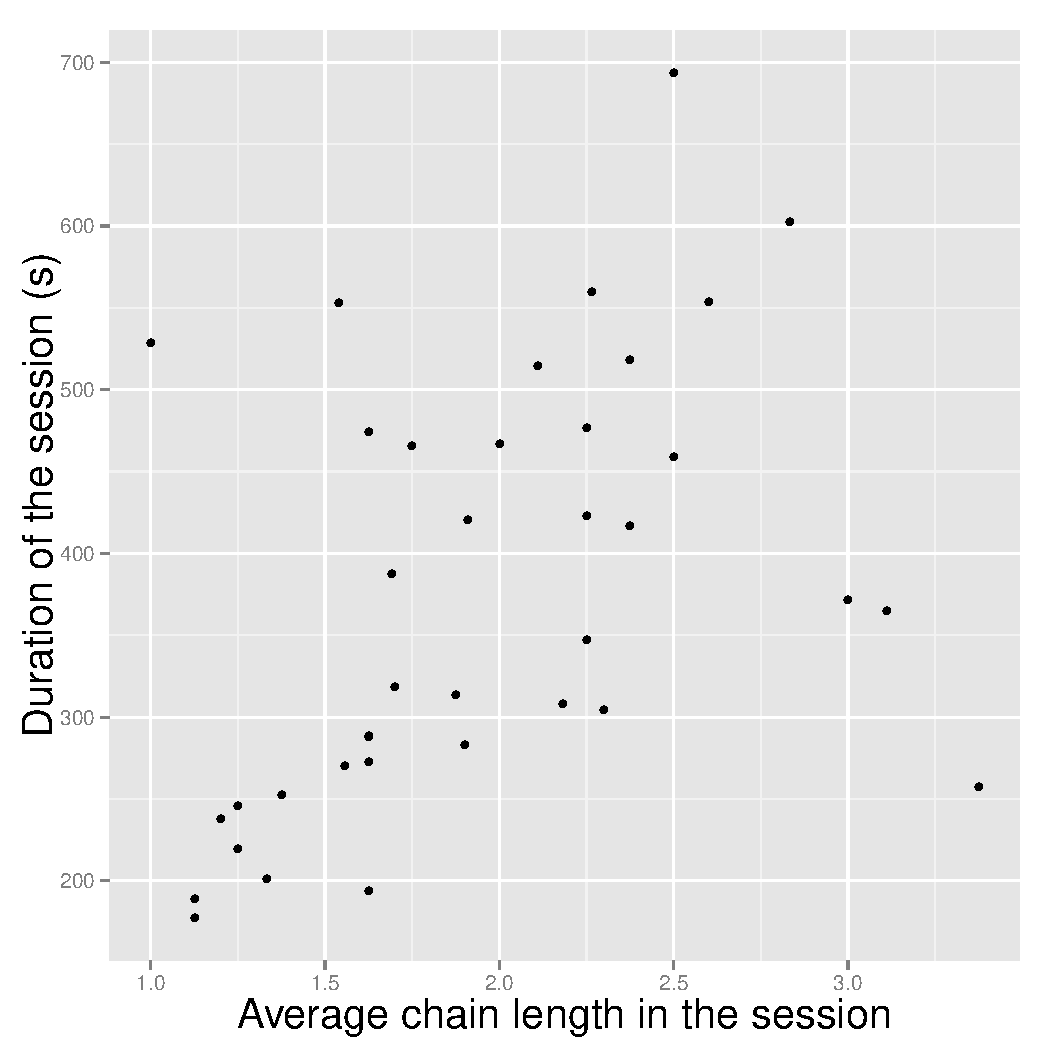
\includegraphics[width=0.6\textwidth]{Images/Chains-duration-LR}
	\caption{Scatter plot of duration of the session and average chain length in the session}
	\label{fig:chains_dur_scatter}
\end{figure}

When I applied linear regression $R^2$ was 0.188, which means the average chain length explains very little of the duration variation. If the average chain length was to significantly influence the duration, I would expect much higher $R^2$. The correlation between the duration and average chain length is not low: 0.433, however correlation does not imply causation. Longer chains can be caused by errors of the IF or the IG and the errors are also likely to increase the duration. Based on these facts, I don't believe the chains are harmful phenomenon and it makes sense to proceed with attempting to model them. 

With modeling the chains of references, there are numerous problems to tackle. The simple presence of a chain can be thought of as a classification task. It can be interesting to try to predict the chain length. Having established common linguistic functions of the chains, classifying chains whether they would contain these functions is another task to consider. I looked into each of these problem. Trough extracting relevant features I thoroughly explored using machine learning for modeling the chains.

As a side note, while exploring chains of references I switched from the Weka implementation of machine learning techniques \citep{hall2009weka} to scikit learn package for Python \citep{scikit-learn}. The main reason was easier automation of the entire pipeline, therefore speeding-up of the whole process and also more control over the whole process.

\subsection{Presence of the chains}
From Subsection \ref{subsec:dataset-chains}, the functions the chains can play in a discourse are known. However, what role does the scene complexity and particular game state play in the presence of the chains? Will more complex scenes spawn more chains or are the chains too complex to be captured by simply looking at where they are created? To answer these question, I extracted scene complexity features and the target button for all references and classified whether a chain was present or not.

The features I extracted from the dataset are in the following list:

\begin{itemize}
\item
Target button	
\item
Number of objects in the room - Figure \ref{fig:chains-distrib-objects}
\item
Number of buttons in the room - Figure \ref{fig:chains-distrib-buttons}
\item
Number of landmarks in the room - Figure \ref{fig:chains-distrib-landmarks}
\item
Number of very close buttons to the target button (closer than 0.3m) - Figure \ref{fig:chains-distrib-veryclose}
\item
Number of buttons on the same wall as target button - Figure \ref{fig:chains-distrib-samewall}
\item
Number of close buttons to the target button (closer than 1m) - Figure \ref{fig:chains-distrib-close}
\item
Number of far buttons (farther than 1.5m) - Figure \ref{fig:chains-distrib-far}
\end{itemize}

The target button is a categorical feature, so I used DictVectorizer class in scikit to transform it into multiple numerical features. I further tried to use all features,to  select the 8 best features using the SelectKBest class from scikit with the $\chi^2$ statistic as a scoring function and to select the 16 best features using the same strategy. As algorithms I used Decision Trees, Naive Bayes, Support Vector Machines (SVM), One-Nearest Neighbour (1-NN), Two-Nearest Neighbours (2-NN) and Random Forest. This selection employs various approaches to classification tasks, each of the algorithms having strong and weak points. For evaluation, I used standard ten-fold cross validation and compared the mean accuracy of the classifiers with the majority class baseline. From now on, I will also include the standard deviation (std) of the accuracy. The results are summarized in Table \ref{tab:chains-ml-presence}. 

\begin{table}[!htbp]
 \centering
\begin{tabular}{lccc}
\toprule
Features & Model    & Mean accuracy (\%) & std \\
\midrule
Majority baseline &    & 55.2	& \\
\midrule
All & Decision Tree 	& 55.5		& 6.8 	\\
	& Naive Bayes  	& 55.8		& 3.3 	\\
	& SVM 			& 56.1		& 5.6  	\\
	& 1-NN			& 56.3		& 4.7 	\\
	& 2-NN			& 53.6		& 6.1 	\\
	& Random Forest	& 55.0		& 6.8	\\
\midrule
8 best 	& Decision Tree 	& 	59.7		& 7.3  	\\
		& Naive Bayes  	&	56.4		& 1.5 	\\
		& SVM 			&	58.3		& 6.6 	\\
		& 1-NN			&	58.8		& 5.6 	\\
		& 2-NN			&	56.1		& 7.2 	\\
		& \textbf{Random Forest}	&	\textbf{60.0	}	& 8.3 	\\
\midrule
16 best & Decision Tree 	& 55.8	& 6.8  	\\
	& Naive Bayes  		& 56.4	& 1.5 	\\
	& SVM 				& 58.3	& 7.0  	\\
	& 1-NN				& 56.9	& 4.6  	\\
	& 2-NN				& 53.3	& 6.4  	\\
	& Random Forest		& 57.2	& 6.4  	\\	
\bottomrule
\end{tabular}
\caption{Results of chains presence modeling}
\label{tab:chains-ml-presence}
\end{table}

The best mean accuracy had the Random Forest for 8 best features. However, it wasn't significantly better than the majority class baseline. Taking into account the standard deviation, none of the classifier and features combination outperformed the baseline.  From these results, I conclude that the chains presence is not dependent only on the scene complexity and specific scenarios. IG strategies for referencing, IF behaviour and other circumstances play role in the creation of the chains.

\subsection{Chain length prediction}
After not being able to predict presence of the chains based on spatial information and the target button, I was interested if I could predict the chain length. I used the same attributes as in the previous classification of the chains' presence, but added two more features concerned with IF movement behaviour. Namely, the ratio of the time the IF spent not moving at all through the chain duration and ratio of the time IF spent only rotating in place through the chain duration. The idea behind these features is that an IF who is not moving or just looking around is an indication of him/her being confused, which then should produce more referring expression for the chain.

For reference, I list all features and add figure numbers for the two new attributes:
\begin{itemize}
\item
Target button	
\item
Number of objects in the room
\item
Number of buttons in the room
\item
Number of landmarks in the room
\item
Number of very close buttons to the target button (closer than 0.3m)
\item
Number of buttons on the same wall as target button
\item
Number of close buttons to the target button (closer than 1m)
\item
Number of far buttons (farther than 1.5m)
\item
Ratio of time IF spent not moving - Figure \ref{fig:chains-distrib-stop}
\item
Ratio of time IF spent rotating - Figure \ref{fig:chains-distrib-rotate}
\end{itemize}

I applied linear regression, predicting chain length based on the three groups of attributes mentioned - the target, spatial features and IF movement behaviour features. I evaluated the regressions by looking at $R^2$. The results are in Table \ref{tab:chains-lr-length}.

\begin{table}[!htbp]
 \centering
\begin{tabular}{lc}
\toprule
Features & $R^2$  \\
\midrule
Target button & 0.154\\
Spatial & 0.146 \\
IF movement & 0.126 \\
Spatial ad IF movement & 0.262 \\
\bottomrule
\end{tabular}
\caption{Results of chains length modeling}
\label{tab:chains-lr-length}
\end{table}

None of the regressions from Table \ref{tab:chains-lr-length} are particularly good at predicting the chain length. Combining spatial and IF movement features does increase the percentage of chain length variation explained by the model, suggesting that these features have, an however small, effect on the chain length. Once again it shows that chains are complex phenomenon, influenced by IF, IG and scene variables.

\subsection{Closer look at chains' content}
Despite not being able to predict the chains presence and length, I was still interested in chains and decided to look closely into the chains content. First, I took advantage of having annotated the functions in the chains, as introduced in Subsection \ref{subsec:dataset-chains}. I focused on the specification and group function and tried to predict whether the chain will contain these functions. Second, I tried to predict whether the chain provides new information about the target button after its first reference. For example the IG could add a RE about the position of the target button relative to a landmark in the third reference of the chain. The reasoning behind this classification is trying to predict when the IG adds information to the chains.

For all these classification tasks, I used the same features as in the chain length prediction, that is: the target button, spatial features, IF movement behaviour features and a combination of the previous two. Again, I used ten-fold cross validation for evaluation and compared that to the majority class baseline. The results for the specification function are in Table \ref{tab:chains-ml-specification}, for the group function in Table \ref{tab:chains-ml-group} and for predicting new information in Table \ref{tab:chains-ml-infgain}. As algorithms, I maintained a broad range of algorithms, similarly to the previous machine learning attempts.

\begin{table}[!htbp]
 \centering
\begin{tabular}{lccc}
\toprule
Features & Model    & Mean accuracy (\%) & std (\%) \\
\midrule
 Majority baseline &   & 74.7	& \\
\midrule
Target button 	& Decision Tree 	& 73.3		& 3.0 	\\
				& Naive Bayes  	& 38.0		& 11.2	\\
				& SVM 			& 74.7		& 1.7	\\
				& 1-NN			& 70.7		& 7.4 	\\
				& Random Forest	& 74.0		& 3.6	\\
\midrule
IF movement	& Decision Tree 	& 	64.0	& 10.9 \\
			& Naive Bayes  	&	72.7	& 5.6	\\
			& SVM 			&	74.7	& 2.7 	\\
			& \textbf{1-NN}	&	\textbf{77.3	} & 6.1 	\\
			& Random Forest	&	71.3	& 8.5 	\\
		
\midrule
Spatial	 	& Decision Tree 	& 74.7	& 8.4 \\
			& Naive Bayes  	& 66.7 	& 10.4	\\
			& SVM 			& 71.3	& 7.4 	\\
			& 1-NN			& 68.7	& 12.0 \\
			& Random Forest	& 74.7	& 9.4 \\	
\midrule
Spatial and movement& Decision Tree 	& 66.7	& 11.6 \\
					& Naive Bayes  	& 66.7	& 10.4	\\
					& SVM 			& 71.3	& 9.5 	\\
					& 1-NN			& 76.7	& 4.5 \\
					& Random Forest	& 68.0	& 8.4 \\			
\bottomrule
\end{tabular}
\caption{Results of specification function in chains modeling}
\label{tab:chains-ml-specification}
\end{table}

\begin{table}[!htbp]
 \centering
\begin{tabular}{lccc}
\toprule
Features & Model    & Mean accuracy (\%) & std (\%) \\
\midrule
Majority baseline &   & 75.4	& \\
\midrule
Target button 	& Decision Tree 	& 81.3		& 7.2 	\\
				& Naive Bayes  	& 38.0		& 7.4	\\
				& SVM 			& 75.3		& 3.1 	\\
				& 1-NN			& 79.3		& 7.0 	\\
				& Random Forest	& 79.3		& 8.7	\\
\midrule
IF movement	& Decision Tree 	& 	61.3	& 11.9 \\
			& Naive Bayes  	&	75.3	& 3.1	\\
			& SVM 			&	75.3	& 3.1 	\\
			& 1-NN			&	73.3	 & 7.9 	\\
			& Random Forest	&	68.0	& 8.4 	\\
\midrule
Spatial	 	& Decision Tree 	& 80.0	& 5.2 \\
			& Naive Bayes  	& 77.3 	& 9.1	\\
			& SVM 			& 77.3	& 4.4 	\\
			& 1-NN			& 77.3	& 6.8 \\
			& \textbf{Random Forest}	& \textbf{82.0}	& 6.7 \\	

\midrule
Spatial and movement& Decision Tree 	& 71.3	& 8.5 \\
					& Naive Bayes  	& 78.0	& 7.9	\\
					& SVM 			& 77.3	& 4.4 	\\
					& 1-NN			& 79.3	& 4.7 \\
					& Random Forest	& 74.0	& 9.2 \\	 	
\bottomrule
\end{tabular}
\caption{Results of group function in chains modeling}
\label{tab:chains-ml-group}
\end{table}

\begin{table}[!htbp]
 \centering
\begin{tabular}{lccc}
\toprule
Features & Model    & Mean accuracy (\%) &  std (\%) \\
\midrule
 Majority baseline  &   & 67.3	& \\
\midrule
Target button 	& Decision Tree 	& 68.3	& 9.8 	\\
				& Naive Bayes  	& 38.0	& 7.9	\\
				& SVM 			& 67.3	& 2.0 	\\
				& 1-NN			& 56.0	& 15.6 	\\
				& Random Forest	& 68.0	& 8.8	\\
\midrule
IF movement	& Decision Tree 	& 	58.7	& 4.0 \\
			& Naive Bayes  	&	68.0	& 5.8	\\
			& SVM 			&	67.3	& 2.0 	\\
			& 1-NN			&	41.3	& 10.3 	\\
			& Random Forest	&	57.3& 6.1 	\\
			
\midrule
Spatial	 	& Decision Tree 	& 68.0	& 8.4 \\
			& Naive Bayes  	& 60.7 	& 14.2	\\
			& SVM 			& 71.3	& 4.3 	\\
			& 1-NN			& 59.3	& 11.0 \\
			& Random Forest	& 67.3	& 8.7 \\	

\midrule
Spatial and movement& Decision Tree 	& 66.0	& 13.2 \\
					& Naive Bayes  	& 62.7	& 13.1	\\
					& \textbf{SVM} 	& \textbf{72.7}	& 4.7 	\\
					& 1-NN			& 59.3	& 9.7 \\
					& Random Forest	& 64.7	& 9.5 \\	 	
\bottomrule
\end{tabular}
\caption{Results of new information in chains modeling}
\label{tab:chains-ml-infgain}
\end{table}

The best classifiers for these 3 tasks can be found in the respective results tables, marked by bold font. Similar to the previous attempts, all combinations of attributes and algorithms had an accuracy around the baseline. The last section of this chapter will address these and all previous results in more depth. But before that, I modeled one more subtask, which is introduced in the following section

\section{Room memory}
\label{sec:room-memory-ml}
The last machine learning problem I tackled was using memory of the previously visited rooms in the RE for room switching. When the IF has to return to a recently visited room, the IG sometimes employs REs such as: ``Go to the room you were just in.'' Deciding whether to use memory in room switching RE can be thought of as a classification task.

I extracted all moments where the IF went between rooms and determined whether the room memory was used from what the IG was saying before going into the new room. I also extracted 3 features:

\begin{itemize}
\item
Was IF in the new room before?
\item
How many seconds before, was he/she there?
\item
How many rooms before, was he/she there?
\end{itemize}

The last feature being of a categorical character, once again DictVectorizer was used for transformation and from the transformed numerical values I selected the 3 best with SelectKBest and the $\chi^2$ statistic. The results are in Table \ref{tab:history-ml}.

\begin{table}[!htbp]
 \centering
\begin{tabular}{lcc}
\toprule
Model    & Mean accuracy (\%) & $2\times$ std (\%) \\
\midrule
 Majority baseline    & 78.5	& \\
\midrule
 Decision Tree 	& 78.0	& 7.1 	\\
 Naive Bayes  	& 68.3	& 7.3	\\
 SVM 			& 82.2	& 6.2 	\\
 1-NN			& 80.8	& 6.6 	\\
 \textbf{Random Forest}	& \textbf{84.4}	& 6.6	\\
\bottomrule
\end{tabular}
\caption{Results of room memory modeling}
\label{tab:history-ml}
\end{table}

Despite not being able to significantly outperform the baseline using machine learning, I used the knowledge gained in the room memory modeling attempt. In the systems I developed for the experiment, which will be discussed in the last chapter, I created a simple rule for using room memory and enhanced the REG process.

The next section analyses results from previous sections and provides my thoughts on them.

\section{Thoughts on machine learning in the S-GIVE dataset}
Thanks to better availability of annotated corpora, machine learning techniques are becoming popular in the field of REG, examples being mentioned in Section \ref{sec:relwork}. Inspired by similar research, I looked into a S-GIVE dataset, so far unexplored using ML, a dataset of spoken instruction giving in 3D virtual environment.

Despite my feature extraction and tackling various problems, the results were unsatisfactory. In this section, I would like to present my thoughts, why I believe that was the case.

First point to explore is the complexity of the S-GIVE scenario. As was already discussed in Section \ref{sec:timing-firsref-ml}, the S-GIVE worlds have specific properties, which most likely have significant influence on the way the IGs formulate their instructions. The S-GIVE dataset is specific in the high frequency of distractors, especially of the same category as the target of the references. To identify targets in such an environment often requires taking into account relations between entities. This was one of the original constrains of early REG research, as mentioned in Section \ref{sec:bg-reg}, and only recently this constraint was attempted to be lifted. In some scenarios, the buttons were intentionally organized in complex arrays, where even the IG wasn't sure which button needs to be pressed. Relatively simple spatial features, which proved to be effective in research of \citet{stoia2006sentence}, likely loose their predictive power when dealing with situations of frequent distractors of the same type as the target.

The dataset size has to be taken into account, when discussing the ML results. The relatively small number of participants and, on the other hand, higher number of scenarios, where REs were created, is something to consider. With a smaller number of participants, the IGs' personal strategies of referring will play a bigger role in the dataset. Some might prefer to refer to the target button immediately, while others might postpone the reference until they removed more distractors through other movement instructions. This difference obviously make any attempts of machine learning difficult on a small dataset. With enough data it would be possible to separate strategies to clusters and examine each cluster separately. However with 20 participants, this is not possible or very difficult to achieve. These strategies are also likely to be influenced by the IFs, further increasing the uniqueness of the REs produced for each pair of IG and IF. I strongly believe a bigger dataset would be more successful in applying ML techniques.

Last but not least, there is a question of the features used. Spatial features are easier to extract from S-GIVE dataset than any other. While I attempted using other features apart from the spatial ones, their extraction is problematic and time consuming. I would speculate that features about the IF's behaviour and the IG's personality might increase accuracy of presented models, but exploring them was beyond the scope of this thesis. Not to mention that some interesting features of a more personal character don't necessarily have to be in the dataset at all and one would have to repeat the experiment to collect them.

That being said, the ML attempts inspired the systems I used in the experiment described in the following chapter in many ways. 




